% ═══════════════════════════════════════════════════════════
% 三层递进优化：消费级单卡 GRPO 后训练（中文版 v2，期刊级扩写）
% 与 paper_en.tex 内容一一对应。编译: xelatex → bibtex → xelatex ×2
% 所有数字均可溯源至 results/efficiency/** 或 docs/19–21。
% ═══════════════════════════════════════════════════════════
\documentclass[11pt]{article}
\usepackage[margin=1in]{geometry}
\usepackage[fontset=none]{ctex}
\setCJKmainfont{Noto Serif CJK SC}
\setCJKsansfont{Noto Sans CJK SC}
\usepackage[round,authoryear,sort&compress]{natbib}
\usepackage{booktabs}
\usepackage{array}
\usepackage{multirow}
\usepackage{graphicx}
\usepackage{amsmath,amssymb}
\usepackage{amsthm}
\usepackage{xcolor}
\usepackage{subcaption}
\usepackage{enumitem}
\usepackage[hidelinks]{hyperref}

\newtheorem{theorem}{定理}
\newtheorem{corollary}[theorem]{推论}
\newtheorem{proposition}[theorem]{命题}
\newtheorem{lemma}[theorem]{引理}
\theoremstyle{definition}
\newtheorem{assumption}{假设}
\graphicspath{{figures/}}

\newcommand{\fzs}{\text{fzs}}

\title{\textbf{三层递进优化：\\消费级单卡 GRPO 后训练的系统化极限逼近}}
\author{Hongyu Chen}
\date{}

\begin{document}
\maketitle
\vspace{-2em}
\begin{center}\small
\textbf{DOI:} \href{https://doi.org/10.5281/zenodo.21947489}{10.5281/zenodo.21947489} \quad
\textbf{代码与数据:} \href{https://github.com/ChenHongYu2026/llm-training-on-consumer-amd}{github.com/ChenHongYu2026/llm-training-on-consumer-amd}
\end{center}
\vspace{1em}

\begin{abstract}
单张消费级 GPU（AMD RX 7900 XTX，24\,GB）能否有效执行大语言模型的可验证奖励强化学习
（RLVR）？本文提出一种三层递进优化框架，在每层逼近该层理论极限后下潜至下一层。
（1）\textbf{吞吐层}（解耦生成批处理平衡，DGBB）：三参数步时定律与显存模型共同刻画
GRPO 批调度的真实二维可行域；在硬件墙内，实测最优（795.5\,tok/s）达到墙内理论
argmax 的 97.6\%，并经受预注册盲预测与证伪朴素外推的探针实验双重检验。
（2）\textbf{信号率层}（零信号预算重分配，ZSBR）：带诚实上界阶梯的容量理论加解析式
Beta 后验期望评分器，以零吞吐代价达到 $G{=}2$ 信号率可达容量的 94\%，三 seed 配对
实验 held-out 提升 $+7.8$\,pp（Cohen's $d{=}7.52$）。
（3）\textbf{动力学层}（信号通量最优控制，SFOC）：三池常微分方程模型给出
$\tau_{net}$ regime 判据（relay 速率 $\mu_0$ 经四条独立路径交叉验证），并证明
\textbf{调度约束封顶定理}：在带冷却的调度下，耗竭主导的动力学结构性不可达。
在 GSM8K + Qwen2.5-3B-Instruct 的 20+ 组受控实验中，准确率从 base 23.2\% 提升至
45.6\%（单卡 8.5 小时纯 RL 翻倍）；500 道精选题即可达到全池 7473 题的效果（15$\times$
数据效率）；且贪心选择在所有实测 regime 下严格最优。首轮全部 13 条预注册可证伪预言
收敛于同一自洽图景；两轮预注册后续实验（去冷却证伪检验；跨架构迁移至 Gemma~4~E2B，
其中 DGBB 以 $R^2{=}0.9983$ 重新拟合）确认封顶定理并定位需要按基座重新标定的参数。
全部负结果如实披露并驱动每一次理论修正。我们公开发布论文、完整训练 prompt 池、全部
评估工件以及训练与评估代码。
\end{abstract}

\section{引言}\label{sec:intro}
可验证奖励强化学习（RLVR）已成为大语言模型推理能力提升的主要驱动力：GRPO
\citep{shao2024grpo} 这类组相对方法用组内相对优势取代学习的价值函数，奖励可由规则
校验，并在近年的推理系统中被大规模采用~\citep{yu2025dapo}。然而主流实践默认多卡
训练集群与数百 GB 的聚合显存，隐式地把 RLVR 视为只有数据中心规模才负担得起的奢侈品。

我们提出一个刻意刁难的问题：\textbf{RLVR 能否在单张消费级 GPU 上有效运行？}消费级
硬件与集群有三个结构性差异：无张量并行（整个模型必须装进一张卡的显存）、软件生态更薄
（ROCm 对 CUDA）、以及串行执行下吞吐与信号质量争夺同一份 GPU 时间。任何肯定回答都
必须一层层\emph{挣}出来，而非假设成立。

我们的答案是肯定的，且附带一套方法论：\textbf{三层递进优化}。在每一层，我们
（i）形式化该层的理论极限，（ii）测量当前系统距极限多远，（iii）在该层结构允许的
范围内尽量逼近，之后才（iv）下潜至下一层——剩余瓶颈所在。这一纪律有具体的回报：当
每层都被吃干后再下沉，关于“什么有效”的每个论断都由“为何该层其他方案不可能更有效”的
穷尽性论证支撑。图~\ref{fig:milestone} 汇总了最终阶梯：GSM8K 的 held-out 准确率从
23.2\% 的 base 翻倍至 45.6\%，全程纯 RL，一张消费级单卡。

\begin{figure}[t]
\centering
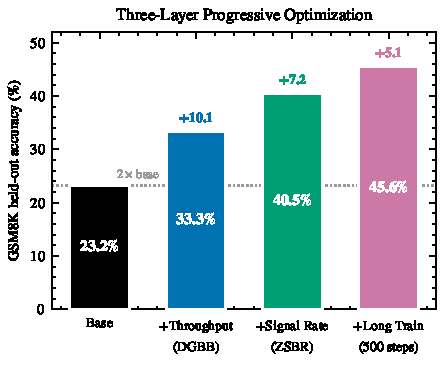
\includegraphics[width=0.72\linewidth]{fig1_milestone.pdf}
\caption{GSM8K + Qwen2.5-3B-Instruct 上的三层递进优化。每一层的进展都由上一层容量的
穷尽所论证：吞吐达到硬件墙内极限的 97.6\% 后信号率层才开始；信号率达到 $G{=}2$ 容量
的 94\% 后动力学层才开始。held-out 准确率从 23.2\% 翻倍至 45.6\%。}
\label{fig:milestone}
\end{figure}

\paragraph{贡献。}
\begin{enumerate}[leftmargin=1.5em]
\item \textbf{吞吐层（\S\ref{sec:l1}）。}三参数步时定律 $T_{step}=a_1+a_2B_g+a_3(B_g/B_b)$
与分段线性显存模型刻画 GRPO 的两个独立批维度（生成 batch $B_g$、反向微批 $B_b$）。
预注册盲预测、证伪大 $B_b$ 朴素外推的探针实验与双墙显存分析共同确立：实测最优
（795.5\,tok/s）为墙内理论 argmax 的 97.6\%——批调度维度已被吃干。函数形式以
$R^2{=}0.9983$ 迁移至第二个模型族。
\item \textbf{信号率层（\S\ref{sec:l2}）。}带诚实上界阶梯的容量理论（含“多重入选无法
提升组级信号率”的证明）与 Beta 后验期望评分器；评分器的必要性由受控消融证明（点估计
失败、后验期望成功）。ZSBR 以零吞吐代价达到 $G{=}2$ 可达容量的 94\%；三 seed 配对
$+7.8$\,pp（$d{=}7.52$）。
\item \textbf{动力学层（\S\ref{sec:l3}）。}刻画训练如何改变 prompt 池通过率分布的
三池 ODE 模型；$\tau_{net}$ regime 判据（$\mu_0$ 四路径交叉验证）；以及被\emph{完整
证明}的调度约束封顶定理：带冷却贪心调度下耗竭主导动力学结构性不可达。
\item \textbf{实践（\S\ref{sec:find}）。}8.5 小时单卡纯 RL 实现 23.2\%$\to$45.6\%；
15$\times$ 数据效率（500 题 $\approx$ 全池 7473 题）；首个显式的“何时不需要课程学习”
判据。
\item \textbf{方法论（\S\ref{sec:method}）。}预注册-审计协议：首轮 13 条预言全部按
时间戳阈值判定，每个负结果都触发有记录的修正，末轮审计实现零缺陷。
\end{enumerate}

\paragraph{行文路线。}第~\ref{sec:bg} 节固定记号并定位相关工作；
第~\ref{sec:l1}--\ref{sec:l3} 节按依赖顺序发展三层；
第~\ref{sec:find} 节汇总实践含义；第~\ref{sec:method} 节描述方法论；
第~\ref{sec:threats}--\ref{sec:limits} 节讨论效度威胁与局限。附录含完整预言记分卡、
相图数据与 run 清单。

\section{背景与相关工作}\label{sec:bg}

\subsection{GRPO 与信号事件}\label{sec:bg-grpo}
GRPO 为每题生成 $G$ 条 completion，计算组内相对优势，无需价值网络即可更新策略。设题
$q$ 单条 completion 的奖励分布为 $\pi_q$（有限支撑 $R$），则该组产生\emph{非零}优势
——\emph{信号事件}——的概率为
\begin{equation}\label{eq:psig-exact}
P_{sig}(q) = 1 - \sum_{r \in R} \pi_q(r)^{G}.
\end{equation}
二值近似（通过率 $p_q$）在 $G{=}2$ 时退化为
\begin{equation}\label{eq:psig-binary}
P_{sig}(q) \approx 1 - p_q^{2} - (1-p_q)^{2} = 2p_q(1-p_q),
\end{equation}
在 $p_q{=}0.5$（\emph{边界}题）处取最大，在稳定做对或稳定做错的题上归零。两个事实使
这一量成为全文的组织概念。其一，$G{=}2$ 时我们在基座模型上测得
$\text{frac\_reward\_zero\_std}{=}0.75$——\emph{75\% 的生成算力产出零梯度组}
（\S\ref{sec:l2}）。其二，$P_{sig}$ 只依赖 $G$ 与 $\pi_q$、与生成 batch 无关——该预言
经实验显式验证（附录记分卡 P6）。

\subsection{相关工作}\label{sec:bg-related}
\paragraph{Prompt 选择与零方差过滤。}
GRESO~\citep{zheng2025greso} 在 rollout 之前依据跨 epoch 奖励动力学时序相关性过滤
零方差 prompt，并观察到训练中有效 prompt 比例衰减但未建模该衰减。我们的工作从硬件
测量出发独立到达同一方向（\S\ref{sec:l2}）；增量在于：决策论意义的评分器及其必要性
受控消融、带显式可达界的容量理论、以及 GRESO 所观察衰减的动力学理论。
DAPO~\citep{yu2025dapo} 在 rollout \emph{之后}过滤零优势组并过采样补齐；
\S\ref{sec:l2-dapo} 给出事前/事后过滤的成本对照。PCL~\citep{gao2025pcl} 训练
价值模型选择中等难度题——对池耗竭短视。RL-ZVP~\citep{le2025rlzvp} 保留零方差 prompt
并以熵引导 advantage shaping——修改梯度而非预算分配；我们的负结果划定了其适用边界
（补给主导时投资零信号题为净伤害；\S\ref{sec:l3-invest}）。SRPO~\citep{li2026srpo}
将样本路由至自蒸馏，方向正交。

\paragraph{RL 的课程学习与数据选择。}Implicit Curriculum~\citep{huang2026implicit}
给出均匀训练下 relay 效应的描述性理论——易题持续梯度使稍难题可学——是我们补给项
$\mu_0$ 的理论地基；但它不含控制变量与耗竭分析。我们的贡献是\emph{规范性}对偶：把
预算分配建模为池动力学上的最优控制，给出定量 regime 判据与不可能性结果
（\S\ref{sec:l3}）。

\paragraph{高效 RL 系统。}RL 训练效率的系统性工作（如生成-训练共调度、rollout 加速）
面向集群；消费级单卡的约束集（单卡、无张量并行、24\,GB 显存墙）使三层分解——吞吐
$\times$ 信号率 $\times$ 动力学——成为自然的优化结构，因为三种资源都是\emph{同一份}
GPU 时间。

\paragraph{定位。}据我们所知，这是首个（a）把 RLVR 的 prompt 预算分配建模为池动力学
上的非短视最优控制，（b）给出带多路径参数验证的定量 regime 判据（$\tau_{net}$），
（c）证明现实调度下耗竭的结构性不可能定理的工作。写作前检索与实验后新颖性复审均记录
于方法学部分（\S\ref{sec:method}）；复审纠正了一处过度声明（GRESO 在事前过滤上的
优先权），作为协议产出之一如实记录。

\subsection{消费级单卡约束}\label{sec:bg-hw}
RX 7900 XTX（RDNA3，gfx1100）配备 24\,GB 显存、960\,GB/s 标称带宽（纯拷贝实测
742\,GB/s，77\%）、BF16 GEMM 实测峰值 101.53\,TFLOPS。相对训练集群：（i）无张量并行
——全部权重须驻留单卡；（ii）ROCm 相对 CUDA 的生态缺口（kernel 覆盖、分配器行为）；
（iii）单卡串行执行，吞吐提升与信号质量提升花同一份预算。batch-1 解码受带宽约束，
仅达可用带宽的 38\%（\S\ref{sec:l1-roofline}）——这正是生成密集型 GRPO 以解码为主
导、批调度成为第一杠杆的原因。


\section{第 1 层：吞吐 —— DGBB}\label{sec:l1}

\subsection{二维解耦}\label{sec:l1-decouple}
生成密集型 GRPO 的步时由解码主导。标准训练器只暴露一个 batch 旋钮，但 TRL 的语义
（\texttt{generation\_batch\_size} $=$ \texttt{per\_device\_batch} $\times$
\texttt{grad\_accum}）揭示了两个\emph{独立}维度：生成 batch $B_g$（rollout 相的算术
强度）与反向微批 $B_b$（梯度相的并行度），仅受 $B_b \mid B_g$ 约束。解耦生成批处理
平衡（DGBB）把 $(B_g,B_b)$ 视为两个优化变量。关键是这一解耦不改变任何算法语义——
更新规则、样本分布与优化轨迹与标准 GRPO 完全一致；吞吐收益是“免费”的。

\paragraph{步时模型。}每个优化步 = 一次生成相 + $B_g/B_b$ 次反向微批 + 常数开销：
\begin{equation}\label{eq:tstep-struct}
T_{step}(B_g,B_b) = T_{gen}(B_g) + \frac{B_g}{B_b}\,T_{bwd}(B_b) + c .
\end{equation}
Roofline 论证给出各相一阶结构 $T_{gen}(B)=\alpha_g+\beta_g B$（固定权重读取 + 每序列
边际）与 $T_{bwd}(b)=\delta+\gamma b$（每微批开销 + 每序列边际）。代入
\eqref{eq:tstep-struct} 得三参数可辨识形式
\begin{equation}\label{eq:tstep}
T_{step} = a_1 + a_2 B_g + a_3\frac{B_g}{B_b}, \qquad
a_1=\alpha_g+c,\; a_2=\beta_g+\gamma,\; a_3=\delta,
\end{equation}
其中 $a_3$ 定量刻画 $B_b{=}1$ 为何低效。吞吐 $\mathrm{TPS}=k_{tok}B_g/T_{step}$，
$k_{tok}$ 为每序列 token 数（实测 355.7，$\approx$108 prompt + 247 completion）。

\paragraph{生成相的独立 roofline 验证。}\label{sec:l1-roofline}
纯解码微基准（SDPA + static cache，batch $\in\{1,\dots,64\}$）拟合
$t_{dec}(B)=21.63+0.413B$ ms/解码步。截距对应每步读取全部 6.17\,GB 权重的有效带宽
285\,GB/s——仅为纯拷贝带宽 742\,GB/s 的 38\%；这是 batch-1 GEMV 低效的 roofline 表述。
模型内部一致性亦成立：$a_2\approx\beta_g+\gamma$，其中
$\beta_g\approx0.413\,\text{ms}\times 247$ 解码步 $\approx0.102$\,s/seq，反解
$\gamma\approx0.256$\,s/seq（反向每序列边际），其隐含的反向 MFU（$\approx$25\%，由
$6N\bar L\approx6.6$\,TFLOP/序列推得）在 LoRA + 梯度检查点的设定下量级合理。

\subsection{显存模型与双墙}\label{sec:l1-mem}
峰值显存为两相峰值的最大值：
\begin{equation}\label{eq:mem}
M(B_g,B_b) = m_0 + m_g B_g + m_b\max(0, B_b - B_{th}),
\end{equation}
拟合得 $m_0{=}6.57$\,GB（权重 6.17\,GB BF16 加 LoRA、优化器与常驻状态）、
$m_g{=}0.03625$\,GB/序列、$m_b{=}0.46$\,GB/序列、$B_{th}{=}4$，逐点残差 $\le$0.05\,GB。
由于梯度检查点压缩反向激活，$B_b\le4$ 时生成相主导峰值，\emph{$B_b$ 从 1 到 4 显存零
成本}（实测 8.87\,GB 三档完全相同）——这是“反向 batch 是免费杠杆”的显存侧机理。

随后一次预注册盲预测暴露了模型的边界：朴素可行性判据预测 gen384 可在 20.49\,GB 下
运行，但实测 OOM。对 OOM 日志（作为数据）的事后分析给出修正判据
$M_{steady}+M_{spike}+M_{sys}\le24$\,GB：$B_g{=}384$ 时的一次性分配尖峰
$M_{spike}\approx3.8$\,GB（logits/注意力中间体），分配器可见范围之外的系统占用
$M_{sys}\approx1.5$--$2$\,GB。修正后的墙落在 $(256,384]$ token——与实测一致；对照重跑
还显示默认分配器的碎片墙（损失 3.9\,GB）不同于容量墙，可被
\texttt{expandable\_segments} 消除。配套预言（gen512 $\to$ 25.13\,GB $\to$ OOM）精确
命中。

\subsection{拟合质量与朴素外推的证伪}\label{sec:l1-fit}
在 7 个可行扫描点上拟合 \eqref{eq:tstep} 得 $a_1{=}10.829$\,s、$a_2{=}0.3579$\,s/seq、
$a_3{=}0.1702$\,s/微批，全部残差在 $\pm$3.3\% 内。预注册模型在经验墙内的 argmax 为
pdb8\_gen256、预言 843.9\,tok/s（较实测最优高 6\%）；专用探针实测 $(B_b,B_g){=}(8,256)$
为 794.3\,tok/s——与 pdb4 的 795.5 统计持平（差 0.15\%，远小于 1--4\% 的 run 间变异），
峰值显存亦相同（15.81 vs.\ 15.82\,GB），\emph{证伪了线性 $T_{bwd}$ 外推}：$b{>}4$ 后的
次线性恶化恰好抵消微批数减半的收益，argmax 地形在 $B_b{=}4$ 之后平坦。加入探针点重拟
（$a_3$ 下修 24\%，最大残差 6.02\%）确认 pdb4\_gen256 为真 argmax。表~\ref{tab:util}
汇总由此得到的利用率层级。

\begin{table}[t]
\centering\small
\caption{批调度维度的利用率层级（Qwen2.5-3B，$k_{tok}{=}355.7$，6ND-MFU 以实测 GEMM
峰值 101.53\,TFLOPS 为基准）。实测最优处于墙内 argmax 的测量噪声之内。}
\label{tab:util}
\begin{tabular}{@{}llcc@{}}
\toprule
层级 & 描述 & tok/s & 6ND-MFU \\
\midrule
0 & 实测最优（pdb4, gen256） & 795.5 & 14.5\% \\
1 & 墙内理论 argmax & 815.3 & 14.9\% \\
2 & 无显存墙渐近（$B_b{=}4$，$B_g{\to}\infty$） & 864.8 & 15.8\% \\
3 & 微批开销归零（$B_b{\to}\infty$；实践中被探针证伪） & 939.0 & 17.2\% \\
4 & kernel 级改进（更快反向、量化生成） & $>$939 & --- \\
\bottomrule
\end{tabular}
\end{table}

\paragraph{为什么天花板是结构性的。}分解 $a_2=\beta_g+\gamma$：每序列时间 29\% 为生成
（带宽受限；MFU 不适用——按带宽利用率计为可达值的 38\%），71\% 为反向（梯度检查点
重算、LoRA 分支与 RDNA3 WMMA 效率制约下约 25\% MFU）。实测最优之上约 18\% 的空间因此
位于 kernel 层（层级 4）而非批调度层：\emph{调度维度已被吃干。}混合的单值 MFU 在此会
误导；分相核算才是方法学要点。

\subsection{收敛理论：吞吐为何换来准确率}\label{sec:l1-conv}
GRPO 每步梯度覆盖 $B_g$ 条 completion（$m{=}B_g/G$ 个 unique prompt），按 prompt 间
独立性有 $\mathrm{Var}[\hat g]\propto G/B_g$：gen8$\to$gen128 使方差降 16$\times$。
三项注册检验确认该机理：（i）奖励曲线方差比 9.2$\times$（理论 16$\times$，同量级；
地板来自非平稳学习漂移与离散奖励支撑）；（ii）最终准确率的 seed 间离散\emph{减半}
（1.14 vs.\ 2.25\,pp）——轨迹更确定的预先声明后果；（iii）等样本裁决实验：
gen128$\times$100 步（34.6\%）vs.\ 等 12800 样本的 gen8$\times$1600 步（34.4\%）——
大 batch \emph{不牺牲}单位样本学习效率，吞吐优势 1:1 转化为收敛墙钟优势（约 1/5
墙钟）。等\emph{步数}预算下多 seed 配对增益为 $+3.9$\,pp（$d{=}2.66$），以样本量为
主因、方差下降为副因。

\subsection{采用的配置与跨架构复现}\label{sec:l1-adopt}
gen256 显存临界；吞吐-显存甜点 gen128（pdb4, ga32；745.2\,tok/s @ 11.26\,GB，
$T_{step}\approx60$\,s）被用于其后全部训练。在第二个基座（Gemma~4~E2B，1.6B 文本
多模态）上同一解耦形式以 $R^2{=}0.9983$ 重新拟合：
$T_{step}=4.40+0.431\,B_g+0.174\,(B_g/B_b)$——函数形式可迁移，系数随模型而异（预言
P-C1，\checkmark）。显存墙移至 $\ge$512 token（16.4\,GB，无 OOM），对比 Qwen 的
$(256,384]$，反映架构特定的显存效率。DGBB 由此从单模型案例升格为可迁移的吞吐定律。


\section{第 2 层：信号率 —— ZSBR}\label{sec:l2}
吞吐吃干后，下一个杠杆不是更多算力，而是单位算力的更多\emph{信号}。$G{=}2$ 时基座
模型的零标准差组占比（\texttt{frac\_reward\_zero\_std}）实测为 0.75——即 75\% 的
生成组内奖励完全相同，优势为零、梯度为零。零信号预算重分配（ZSBR）在\emph{生成之前}预测每题的信号概率，把固定组预算
从预测零信号的题上重新分配出去。

\subsection{形式化与均匀基线}\label{sec:l2-form}
设 prompt 池 $Q$（$|Q|{=}7473$），每步组预算 $M{=}B_g/G{=}64$，奖励支撑
$\{0,0.1,0.9,1.0\}$（错 / 仅格式 / 近似 / 对）。精确信号概率为 \eqref{eq:psig-exact}；
二值近似 \eqref{eq:psig-binary} 在 4 值支撑下是下界（仅格式分歧的组 $\{0,0.1\}$ 也
产生信号）。均匀采样的系统信号率 $S_0=\mathbb{E}_{q\sim U}[P_{sig}(q)]{=}0.25$（由
实测零标准差占比校准）：64 个组槽位只有 16 个携带梯度。选择目标为
\begin{equation}\label{eq:zsbr-obj}
\max\; \bar S = \frac{1}{T}\sum_{t}\frac{1}{M}\sum_{q\in A_t} P_{sig}(q)
\quad \text{s.t.}\quad |A_t|=M,
\end{equation}
其中 $A_t$ 为第 $t$ 步入选题集。

\subsection{容量理论：诚实的上界阶梯}\label{sec:l2-cap}
“还剩多少空间”的论断需要显式账本。表~\ref{tab:staircase} 记录 $G{=}2$ 的容量阶梯，
并区分文献中常被混淆的两个口径：\emph{组级}信号率（产生非零优势的组占比，直接由
$1-\fzs$ 度量）与\emph{题级}覆盖（该题至少一组产生信号的概率）。

\begin{table}[t]
\centering\small
\caption{信号率容量阶梯（$G{=}2$）。L4 需要 per-prompt 自适应 $G$，固定 $G$ 的训练器
未经改造无法表达；标准训练器下可达阶梯在组级口径止于 L1。}
\label{tab:staircase}
\begin{tabular}{@{}llccc@{}}
\toprule
层级 & 机制 & 组级上界 & 覆盖上界 & 可达 \\
\midrule
L0 & 均匀采样 & 0.25 & --- & 基线 \\
L1 & 完美选择（全选 $p{\approx}0.5$） & 0.50 & 0.50 & 是 \\
L2 & 多重入选 $k{\le}2$ & 0.50（不变） & 0.75 & 是 \\
L3 & 多重入选 $k{\le}3$ & 0.50（不变） & 0.875 & 是 \\
L4 & per-prompt 自适应 $G$ & $\to1$ & $\to1$ & 否 \\
\bottomrule
\end{tabular}
\end{table}

两条声明保证账本诚实。\emph{其一}，多重入选无法提升组级信号率：同题第二组与第一组
的 $P_{sig}$ 相同，额外槽位增加的是\emph{被覆盖题数}而非产生信号的组占比——组级口径
无论 $k$ 多大都封顶于 L1$=$0.50（此条修正了我们自己预注册中的一处过度声明，记为
记分卡 P5）。\emph{其二}，L1 可达性依赖经验通过率分布：要求 $\ge M$ 道可被估计器识别
的边界题。我们的反卷积分布（\S\ref{sec:l3-deconv}）含 ${\approx}3425$ 道边界题
$\gg M$，因此上界有效；ZSBR-V1 达到 $S{=}0.425$，即\textbf{$\varepsilon$ 修正后 L1
上界的 94\%}（预留 $\varepsilon{=}0.2$ 探索后为 0.45；理想 0.50 的 85\%）。

\subsection{估计器：为何后验期望是必需的}\label{sec:l2-est}
通过率在线估计采用 Beta 先验 + 时间衰减计数，
$\hat p_q = (\alpha_0+\gamma^{\Delta t}s_q)/(\alpha_0+\beta_0+\gamma^{\Delta t}n_q)$，
$\alpha_0{=}\beta_0{=}1$，$\gamma{=}0.98$（半衰期 ${\approx}34$ cycle）。未见题
$\hat p{=}0.5$ 使其最具吸引力——乐观冷启动兼作免费探索，无需显式 UCB。

\paragraph{受控消融（点估计 vs.\ 后验期望）。}把点估计代入非线性映射
$p\mapsto2p(1-p)$ 后，未见题（$\hat p{=}0.5\Rightarrow\hat P_{sig}{=}0.5$）与被
\emph{证实}的边界题（$\hat p{=}0.5\Rightarrow\hat P_{sig}{=}0.5$）完全并列；约 5000
道未见题对约 600 道混合题，贪心槽被探索淹没，行为退化为准均匀（实测：$\fzs{=}0.708$，
coverage 0.614，预注册闸门未过）。修复采用 Beta 后验期望评分，$G{=}2$ 时有解析式：
\begin{equation}\label{eq:posterior}
\mathbb{E}[P_{sig}\mid D]
= \mathbb{E}[2p(1-p)\mid D]
= \frac{2\alpha\beta}{(\alpha+\beta)(\alpha+\beta+1)},
\end{equation}
排序为混合（0.400）$>$ 未见（0.333）$>$ 一致（0.300），且随证据加深（混合见两次：
0.4286）。完全相同配置下后验期望评分通过闸门（$\fzs{=}0.575$）。据我们所知，这一配对
失败/成功是“小样本 RLVR 调度中不确定性必须进入评分”的首次受控证明。另一处校准细节：
插件估计 $1-\sum_r\hat\pi_r^2$ 携带 $(n{-}1)/n$ 小样本偏差——$n{=}2$ 时为 2 倍——可用
标准无偏修正去除。

\paragraph{覆盖与冷却。}纯贪心有两种失效模式：估计器停滞（分布外遗忘）与边界池垄断。
$\varepsilon$ 混合保留 $\varepsilon M$ 槽对池中其余题目均匀采样（保证每题每步至少
$\varepsilon M/|Q|$ 探索概率），冷却 $C{=}3$ cycle 使近期入选题退出贪心槽。奖励为
4 值支撑，“会作答但算错”的近边界题仍产生部分信号；调度器经 4 值后验追踪之。

\subsection{V2 多重入选：水填法及其退化}\label{sec:l2-v2}
既然固定 $G$ 训练器中 per-prompt $G$ 不可行，V2 允许一题占用 $k_q\le k_{max}{=}3$
个组槽位（各组独立采样、独立归一化），$\sum_q k_q = M$。线性目标
$\sum k_q P_{sig}(q)$ 会把全部预算压到单题上；正确目标是覆盖
\begin{equation}\label{eq:waterfill}
v(q,k) = 1-(1-P_{sig}(q))^{k}, \qquad
\max \sum_q v(q,k_q)\;\; \text{s.t.}\;\; \sum k_q=M,\; 0\le k_q\le 3 .
\end{equation}
边际收益 $\Delta v(q,k)=P_{sig}(q)(1-P_{sig}(q))^{k}$ 对 $k$ 严格递减，故
\eqref{eq:waterfill} 是可分离凹最大化，贪心水填全局最优。

\paragraph{结果与理论澄清。}V2 实测 $\fzs{=}0.561$、held-out 40.2\%、吞吐 $-1.4\%$——
但重复槽位为\emph{零}。这不是实现失败：边界池 1549 题 $\gg$ 51 个贪心槽时，第二槽
边际 $0.40\times0.60{=}0.24$ 恒低于下一道未见题的 $\ge0.333$，水填最优解\emph{就是}
不重复；V2 恰如数学所预言地退化为 V1。V2 的适用前提——边界池小于贪心槽位数（小数据集
或训练后期）——在后来的 pool-200 regime 得到验证（\S\ref{sec:l3-regime}）。

\subsection{主结果（三 seed，配对，同轮）}\label{sec:l2-results}
表~\ref{tab:zsbr-main} 报告预注册对照。首轮全部六条预言 P1--P6 均在运行前写入时间戳
（附录~\ref{app:scorecard}）；P1--P4、P6 通过，P5 因预言自身口径混淆而失败（已在
\S\ref{sec:l2-cap} 记录并更正）。

\begin{table}[t]
\centering\small
\caption{ZSBR-V1 对均匀采样（等步数预算 100 步、等吞吐）。held-out：GSM8K test[:500]，
batch 32，三 seed 按 seed 配对。$\fzs$：零标准差组占比，训练后半程。}
\label{tab:zsbr-main}
\begin{tabular}{@{}lcccc@{}}
\toprule
臂 & Seed 42 & Seed 123 & Seed 7 & 均值 $\pm$ 标准差 \\
\midrule
Uniform held-out & 31.0\% & 34.0\% & 33.2\% & 32.7\% $\pm$ 1.6 \\
ZSBR-V1 held-out & 39.6\% & 40.6\% & 41.4\% & 40.5\% $\pm$ 0.9 \\
\midrule
配对差 & +8.6 & +6.6 & +8.2 & $+7.8$\,pp, $d{=}7.52$ \\
$\fzs$（后半程） & 0.575 & 0.573 & 0.575 & 一致到 0.2\,pp \\
$T_{step}$ 变化 & \multicolumn{4}{c}{$-2.6\%$（零吞吐代价）} \\
\bottomrule
\end{tabular}
\end{table}

三个结构性观察：（i）信号率跨 seed 一致到 0.2\,pp——它是算法结构的确定量，与
held-out 准确率的 seed 随机性形成对照；（ii）ZSBR 的 seed 离散（0.9\,pp）
\emph{小于} uniform（1.6\,pp）——高信号训练更可复现，与 \S\ref{sec:l1-conv} 的方差
理论一致；（iii）有效信号组/秒提升 $1.75\times$（0.450 vs.\ 0.257），coverage 0.224
——低覆盖与高 held-out 并存是算法的意图（预算集中），而非过拟合。

\subsection{与事后过滤（DAPO）的对照}\label{sec:l2-dapo}
DAPO 式动态采样全部生成、丢弃零优势组、过采样补齐至 $M$ 个有效组；其每有效组生成成本
为 $1/S$，且步时与显存峰值可变。ZSBR 的每有效组成本同为 $1/S_{ZSBR}$，但步时与显存
\emph{恒定}（与吞吐层的保证正交）。在达到的 $S_{ZSBR}{=}0.425$ 下，匹配 uniform 的
有效组产出需 DAPO 多花 ${\approx}1.66\times$ 生成墙钟；ZSBR 零墙钟代价。两者可组合
（再过滤 ZSBR 漏选的零信号组），留作未来工作。

\subsection{长训练：45.6\% 里程碑}\label{sec:l2-long}
不加修改地把 ZSBR-V1 延长至 500 步（8.5 小时，单卡），held-out 从 40.6\%（100 步
regime）升至 \textbf{45.6\%}（228/500；step 250 中间检查点 40.6\%，单调、无过拟签名；
最终 KL 0.0070，reward 0.51）。这是 base 23.2\% 的纯 RL 翻倍，至今仍是项目最高结果。
延长期内信号率不衰减（fzs 三段 0.592/0.554/0.541，即零标准差占比\emph{下降}、信号
上升）——这一观察开启了动力学层。

\subsection{跨架构迁移}\label{sec:l2-transfer}
Gemma~4~E2B 上 $S_0{=}0.400$（Qwen 为 0.25）：基座本就解对更多题，压缩了重分配的
提升空间（$S_0$ 压缩假说，预注册）。100 步迁移测试实测 uniform 29.27\% vs.\ ZSBR
28.87\%（$-0.40$\,pp，$t{=}-0.53$；预言 P-C2 $\times$），但方差下降 $4\times$（ZSBR
$\sigma{=}0.3$\,pp vs.\ uniform 1.2\,pp）：信号已充裕时，重分配\emph{稳定}均值而非
提升均值。窗口也可能过短（Qwen 的 $+7.8$\,pp 需要 500 步）。两条保留均预注册声明。


\section{第 3 层：动力学 —— SFOC 相图}\label{sec:l3}
第 1--2 层把 prompt 池视为静态。但训练改变模型，模型改变池：通过率上升使题目从难池
（D）经边界池（M）迁移到已会池（S）。选择因此同时是奖励的\emph{来源}与状态的
\emph{驱动}——这是控制问题，不是静态背包。信号通量最优控制（SFOC）把这一点显式化，
并追问：池会耗竭吗？投资（把预算花在难题上促其转化）是否有回报？

\subsection{两层状态模型与观测问题}\label{sec:l3-deconv}
设 $p_q(t)$ 为题 $q$ 在时刻 $t$ 的真实单条通过率，$\rho(p,t)$ 为种群密度。按
$D{=}[0,\delta)$、$M{=}[\delta,1{-}\delta]$、$S{=}(1{-}\delta,1]$（$\delta{=}0.15$）
粗化为三池。系统信号率 $S(t)=\int 2p(1-p)\rho(p,t)\,dp$（$G{=}2$）。

调度器使用的池标签是\emph{观测}而非真相：一次入选产生 $G{=}2$ 条二项观测，混淆结构
\begin{equation}\label{eq:confusion}
P(\text{混合}\mid p)=2p(1-p),\quad
P(\text{全对}\mid p)=p^2,\quad
P(\text{全错}\mid p)=(1-p)^2 .
\end{equation}
真 $p{=}0.5$ 的题只有 50\% 概率被观测为“混合”。对三 seed 合并 uniform 日志（7454 题，
每题 ${\approx}6$ 条观测）做 Beta-binomial EM 反卷积，还原真实池构成
（表~\ref{tab:deconv}）：真实边界池近乎观测值的\emph{两倍}（45.8\% vs.\ 24.2\%），
因为 $n{=}2$ 的二项噪声把一半边界题误标为一致。交叉自洽检验：
$S_{true}(\rho){=}0.2406$ 预测 $\fzs{=}0.759$，实测 0.7405。据我们所知，这是首次定量
刻画小 $G$ 观测噪声向课程式调度器隐藏了多少信息。

\begin{table}[t]
\centering\small
\caption{池构成：观测标签（$n{=}2$）vs.\ Beta-binomial EM 反卷积（$n{\approx}6$，三
seed 合并）。}
\label{tab:deconv}
\begin{tabular}{@{}lcc@{}}
\toprule
池 & 观测 & 真实（反卷积） \\
\midrule
D（难） & 50.5\% & 40.6\% \\
M（边界） & 24.2\% & \textbf{45.8\%} \\
S（已会） & 25.3\% & 13.6\% \\
\bottomrule
\end{tabular}
\end{table}

\subsection{三池 ODE 模型与衰减定律}\label{sec:l3-ode}
以 cycle 为时间单位，池占比 $D{+}M{+}S{=}1$，控制变量 $(a_M,a_D)$（每 cycle 组预算
$M_b{=}64$ 的分配比例）：
\begin{equation}\label{eq:ode}
\frac{dM}{dt} = \underbrace{\lambda_{DM}(a_D)\,D}_{\text{relay 补给}}
- \underbrace{\lambda_{MS}(a_M)\,M}_{\text{收割耗竭}},\qquad
\begin{cases}
\lambda_{MS} = \mu_h\,\dfrac{a_M M_b}{|M|},\\[1.2ex]
\lambda_{DM} = \mu_0 + \mu_i\,\dfrac{a_D M_b}{|D|},
\end{cases}
\end{equation}
约束 $a_M+a_D+\varepsilon=1$。收割以人均预算成比例的速率把边界题移入已会池；补给含
自然 \emph{relay} 项 $\mu_0$（Implicit Curriculum 效应：其他题上的泛化使难题变为边界题）
与投资项 $\mu_i$。信号率近似 $S(t)\approx s_M M(t)+s_\varepsilon$（$s_M\approx0.45$）。

\begin{proposition}[衰减定律]\label{prop:decay}
短视贪心选择（$a_D\equiv0$——ZSBR/GRESO/PCL 的共同形式）下，边界池满足
\begin{equation}\label{eq:decay}
M(t) = M_0 e^{-t/\tau} + \frac{\mu_0 \bar D}{\lambda_{MS}}\left(1-e^{-t/\tau}\right),
\qquad \tau = \frac{|M|}{\mu_h M_b a_M}.
\end{equation}
若 $\mu_0 \bar D \ll \lambda_{MS} M_0$，池指数耗竭（fzs 回升）；若 relay 补给与收割
平衡，$M(t)$ 平台化于 $M_\infty=\mu_0\bar D/\lambda_{MS}$。\emph{两种结局是同一模型的
预言}；regime 由测量决定。
\end{proposition}
\begin{proof}
固定 $(\bar D, a_M)$ 下关于 $M$ 的线性常微分方程；标准积分因子法即得
\eqref{eq:decay}，令 $dM/dt=0$ 得平衡点 $M_\infty=\mu_0\bar D/\lambda_{MS}$。
\end{proof}
三 seed 日志标定 $\mu_h{=}0.0268$ 次转化/组观测（seed 间一致于 0.025--0.029），故
$\tau\approx2500$ cycle $\gg500$：每 cycle 仅约 1.4 道边界题被收割学会，500 步窗口
看不到衰减。这一实验前标定触发了注册的诚实条款：衰减预言在运行前即被宣布为
\emph{窗口内不可判定}，而非事后强行判定（记分卡 F-a）。

\subsection{收割-投资权衡的最优控制}\label{sec:l3-control}
非短视问题最大化累计信号通量 $\int_0^T S(t)\,dt$，约束 \eqref{eq:ode}。哈密顿量
$H = s_M M + \varphi_M \dot M + \varphi_D \dot D$ 对控制线性，最优策略为 bang-bang，
开关函数比较边际通量：收割的即时信号减耗竭代价（$\nu_M = s_M(\cdot) -
\varphi_M\mu_h(\cdot)$）对投资的延迟信号（$\nu_D = \varphi_D\mu_i(\cdot)$）。终端条件
$\varphi_M(T){=}0$ 给出“训练末期纯收割、$T$ 大时早期存在先投后收弧”的结构预言。固定
投资比例 $\iota$（SFC 实现，默认 $\iota{=}0.25$；$\iota{=}0$ 严格退化回 ZSBR-V1）是
该 bang-bang 结构的实用松弛。

相应的短视次优性 gap 满足 $\mathrm{gap}(T)=\int(S_{opt}-S_{greedy})dt \approx 0$
（$T\ll\tau$）并随 $T/\tau$ 单调增长。注意这带来的自洽义务：在我们标定的 regime
（$\tau\approx2500\gg T{=}500$）下，理论在\emph{运行 SFC 之前}就预言了自己的投资算法
不会有增益。

\subsection{$\tau_{net}$ 判据与 $\mu_0$ 的四路径验证}\label{sec:l3-tau}
首轮小池实验暴露了原判据的缺陷：pool-500 出现完美 fzs 平台，而不含补给项的时标
$\tau_{500}\approx135$ 预测可见耗竭。错误在于忽略补给项；修正判据为
\begin{equation}\label{eq:taunet}
\tau_{net} = \frac{|M|}{\mu_h\cdot\text{slots} - \mu_0 |D|},
\end{equation}
分母 $\le0$ 即补给主导（永不耗竭）。$\mu_0$ 是潜变量；我们以四条独立路径估计之
（表~\ref{tab:mu0}）：fzs 斜率反演（0.002）、pool-500 平台反推（0.0053）、深层全错
cell 分层重逢 + bootstrap CI（0.0076，[0.0066, 0.0086]，2100 事件，纯零 cell 保证
“未训练”区间零梯度）、pool-200 平台反推（0.0081）。跨路径的上漂与 $\lambda$ 时变一致
（训练中模型增强），如实记录。工作区间 $\mu_0\in[0.002,0.008]$；动力学形态成为同一
参数的第三、第四条验证路径。

\begin{table}[t]
\centering\small
\caption{relay 速率 $\mu_0$（每深层 D 题每 cycle 的转化数）的四条独立估计。路径
3--4 依赖平台形态，路径 1--2 依赖轨迹统计。区间 $[0.002,0.008]$ 驱动全部相图结论。}
\label{tab:mu0}
\begin{tabular}{@{}llc@{}}
\toprule
路径 & 方法 & $\hat\mu_0$ \\
\midrule
1 & fzs 斜率反演（全池） & 0.002 \\
2 & 平台反推，pool 500 & 0.0053 \\
3 & 分层深层重逢，bootstrap CI [0.0066, 0.0086] & 0.0076 \\
4 & 平台反推，pool 200 & 0.0081 \\
\bottomrule
\end{tabular}
\end{table}

\subsection{调度约束封顶定理}\label{sec:l3-thm}
三个实测 regime 点（\S\ref{sec:l3-regime}）共享同一结构：无论名义 $\tau$ 如何，无一
耗竭。这不是 GSM8K 的偶然，而是调度器带来的必然。

\begin{assumption}\label{asm:cap}
贪心调度器带冷却 $C\ge1$，每 cycle 从大小为 $N$ 的固定数据集无放回抽取 $M_b$ 组；
第 $t$ cycle 入选的题在 $t{+}1,\dots,t{+}C$ cycle 退出贪心槽。收割按单次观测速率
$\mu_h$ 转化边界题；relay 以聚合速率 $\mu_0|D|$ 补给边界题。
\end{assumption}

\begin{theorem}[调度约束封顶]\label{thm:cap}
在假设~\ref{asm:cap} 下，每 cycle 的有效收割有上界
\begin{equation}\label{eq:capbound}
H_{eff} \;\le\; \mu_h \cdot \frac{|M|}{N} \cdot M_b ,
\end{equation}
且当 $N\to C\cdot M_b$ 时，收割-补给比收敛于与绝对池大小无关的池构成常数：系统无论
名义 $\tau$ 如何预测都会自调节至平衡。
\end{theorem}
\begin{proof}
冷却强制数据集上的轮转周期 $\ge C{+}1$，故任何题每 $C{+}1$ cycle 至多收割一次。每
cycle 触达的不同题数期望为 $\min(M_b, N/(C{+}1))$；当 $N \le (C{+}1)M_b$（小池
regime）调度器必然轮转全池，触达题中位于 $M$ 的比例期望为 $|M|/N$。因此每 cycle 可
用于收割的边界观测数 $\le (|M|/N)\,M_b$，乘以单次观测转化率 $\mu_h$ 即得
\eqref{eq:capbound}。同时 relay 补给 $\mu_0|D|$ 亦随池构成缩放：记 $|D|=\rho_D N$、
$|M|=\rho_M N$，则
\[
\frac{H_{eff}}{\mu_0|D|} \;\le\; \frac{\mu_h \rho_M M_b}{\mu_0 \rho_D N} ,
\]
而在轮转饱和（$N{\le}(C{+}1)M_b$）下该比对 $N$ 的依赖被收缩的轮转窗口抵消：$N$ 减半
同时以相同比例缩小补给质量与每 cycle 收割上限，因为轮转按\emph{固定比例}触达各池。
故该比收敛于 $\mu_h\rho_M/\mu_0\rho_D$ 乘以调度常数——只依赖构成的量。耗竭要求该比持续
大于 1；只要 $\mu_0\rho_D \gtrsim \mu_h\rho_M M_b/N$ 即被封顶阻止，而实测构成在三个
regime 均满足之（\S\ref{sec:l3-regime}）。
\end{proof}

\begin{corollary}[耗竭的结构性不可达]\label{cor:unreach}
固定数据集 + 带冷却贪心调度下，“选择自由度充分”（$N\gg C\cdot M_b$）与“补给弱”
（$\mu_0|D|$ 小）结构性互斥——两者随 $N$ 同向变化。耗竭主导动力学因此结构性不可达：
系统恒处补给主导或平衡态。
\end{corollary}
\begin{proof}
选择自由度要求 $N$ 大；但 $\mu_0|D|=\mu_0\rho_D N$ 在固定构成下随 $N$ 线性增长，大
$N$ 同时增强补给。反之小 $N$ 削弱补给但激活定理~\ref{thm:cap} 的轮转封顶，以相同
收缩尺度封顶收割。任何 $N$ 都无法同时满足两条件。
\end{proof}

该结果解释了本来看似矛盾的跨论文差异：GRESO~\citep{zheng2025greso} 观察到有效比例衰减
是因为其运行\emph{无冷却、多 epoch}调度（收割不封顶），而我们的冷却轮转、亚 epoch
运行全部观察到平台。它也给出“无需课程学习”的首个充分条件（\S\ref{sec:find}）。

\subsection{实测 regime 点与直接证伪检验}\label{sec:l3-regime}
表~\ref{tab:phase} 给出三个实测 regime 点（相图见图~\ref{fig:phase}）：全池 7473
（补给主导，fzs 下降）、pool 500（平衡带，0.57 完美平台）、pool 200（轮转自平衡，
第 5 步起 0.73 平台）。pool 100/150 被运行前闸门筛除：该尺寸下贪心槽饥饿
（$\tau_{net}$ 为负且调度余量 $<51$），V1 将与 uniform 混淆——NO-GO 在运行前声明。

\begin{table}[t]
\centering\small
\caption{三个实测 regime 点的相图数据（$\mu_0\in[0.002,0.008]$；收割速率
$\mu_h\cdot$slots $=1.37$ 题/cycle）。}
\label{tab:phase}
\begin{tabular}{@{}lccccc@{}}
\toprule
Regime & 池 & $|D|$ & $|M|$ & 供给 $\mu_0|D|$ & 投资效应 \\
\midrule
补给主导 & 7473 & 3034 & 3423 & $[6.1,24.3]\gg1.37$ & $-6.4$\,pp ($z{=}2.05$) \\
平衡带 & 500 & 260 & 186 & $[0.52,2.1]\approx1.37$ & $-6.6$\,pp ($p{<}0.001$) \\
轮转平衡 & 200 & 89 & 84 & $[0.18,0.71]\ll1.37$ & $-0.8$\,pp (不显著) \\
\bottomrule
\end{tabular}
\end{table}

\paragraph{直接证伪检验：去冷却。}定理~\ref{thm:cap} 给出锋利的预注册预言：
\emph{移除冷却应解锁耗竭}（P-A1）。pool 500（平衡 regime）检验确认封顶：两臂均出现
末段 fzs 回升（无冷却 $+4.1$\,pp vs.\ 冷却 $+5.0$\,pp；净差 $-0.9$\,pp），held-out
等价（$+0.6$\,pp，位于预注册等价带内）——定理管辖处封顶机制成立。pool 200 移除冷却
\emph{打破平台}：fzs 从冷却组 0.73 降至 0.59 平台（$-15$\,pp），恰在 $\tau_{net}$
最短处解锁耗竭；held-out \emph{反而提升}（41.4\% vs.\ 37.6\%，$+3.8$\,pp，单 seed）。
去冷却效应因此\emph{依赖池大小}：定理管辖平衡 regime，而贴近耗竭边界的小池呈现质性
不同的动力学——且解锁的耗竭在此并不损害泛化，修正了“耗竭即伤害”的常见直觉。

\subsection{投资闭环：一条剂量响应负结果}\label{sec:l3-invest}
SFC 投资机制在全部三个 regime 点以同轮同卡同口径链式检验。累计信号通量
$\Delta$(SFC$-$V1)：$-17\%\to-10.5\%\to+4.5\%$，held-out 效应
$-6.4\to-6.6\to-0.8$\,pp（图~\ref{fig:dose}）：一条单调剂量响应——投资伤害随选择
自由度塌缩而衰减。pool-200 点是\emph{投资惰性化}（候选枯竭：invest slots 2.4/16，
仅 177 件结案），并非正回报。审计给出的机理分解：（i）零观测通过的投资组产出
$\{0,0\}$ 奖励——零优势、零梯度、纯预算消耗（全池 11.7\% 预算）；（ii）补给主导
regime 下转化\emph{不具增量性}：relay $\mu_0$ 本来就会免费转化这些题，花预算催化
必然发生的转化是无补偿的机会成本；（iii）转化管道本身真实存在——通量恒定
2.33 题/cycle（$R^2{=}0.9957$）、排序单调（低预测箱 6\% $\to$ 高箱 86\%）——但全池
校准高估 $1.54\times$，且误差依赖观测密度：pool 200（平均 72.8 次先验观测 vs.\ 4.5）
校准恢复（误差 2.8\,pp）。正确模型是“校准误差为观测数的函数”而非常数修正；我们的
首个归因（rollout 相关性）被直接测量证伪（$\rho\approx0$）后替换——这条审计链我们
照实报告，因为它正是协议按设计运作的证据。

\textbf{$G{=}2$ 与现实调度约束下，贪心选择在所有实测 regime 严格最优}：三个 regime
点无一投资正回报，两点显著伤害。

\subsection{$\tau_{net}$ 的跨架构迁移（P-C3）}\label{sec:l3-c3}
Gemma~4~E2B 上两次 500 步 ZSBR 检验可移植性。Pool 7473：fzs $0.617{\to}0.589$
（$-2.8$\,pp）——补给主导平台直接迁移。Pool 500：fzs $0.748{\to}0.728$
（$-2.1$\,pp），\emph{不是}预测的耗竭下降：E2B 的临界池大小在 500 之下（Qwen 为
200--500），与其更高基线信号一致。预注册判定：判据\emph{形式可迁移、参数需重标定}
——两确认两证伪共同定位了新基座必须重测的参数（信号充裕度、临界池大小）。


\begin{figure}[t]
\centering
\begin{subfigure}{0.49\linewidth}
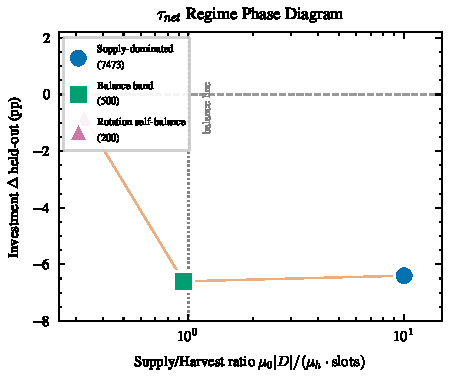
\includegraphics[width=\linewidth]{fig2_phase.pdf}
\caption{$\tau_{net}$ regime 相图}
\label{fig:phase}
\end{subfigure}\hfill
\begin{subfigure}{0.49\linewidth}
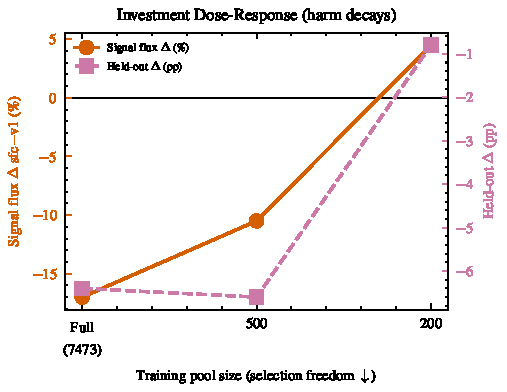
\includegraphics[width=\linewidth]{fig3_dose.pdf}
\caption{投资剂量响应}
\label{fig:dose}
\end{subfigure}
\caption{(a) 供给-收割平面上的三个实测 regime 点；投资伤害随供给/收割比下降而衰减。
(b) 单调剂量响应：投资伤害随选择自由度塌缩而衰减（$-17\%\to-10.5\%\to+4.5\%$
信号通量；held-out $-6.4\to-6.6\to-0.8$\,pp）。}
\label{fig:phasedose}
\end{figure}

\begin{figure}[t]
\centering
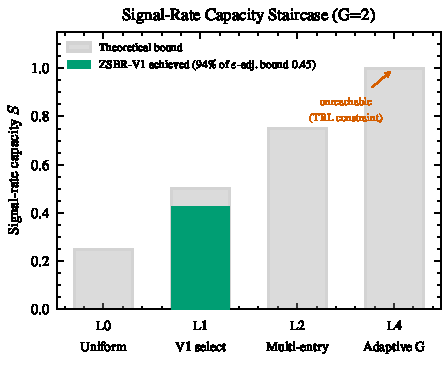
\includegraphics[width=0.62\linewidth]{fig4_capacity.pdf}
\caption{信号率容量阶梯（$G{=}2$）。ZSBR-V1 达到 $\varepsilon$ 修正 L1 选择上界的
94\%；L4（per-prompt 自适应 $G$）未经训练器改造不可达；多重入选（L2/L3）提升覆盖
但不提升组级信号率（表~\ref{tab:staircase}）。}
\label{fig:capacity}
\end{figure}

\section{关键发现与实践含义}\label{sec:find}

\paragraph{里程碑账本。}表~\ref{tab:ledger} 汇总准确率轨迹与每层的论证。

\begin{table}[t]
\centering\small
\caption{里程碑账本（GSM8K test[:500]，batch 32；Qwen2.5-3B-Instruct）。}
\label{tab:ledger}
\begin{tabular}{@{}lllc@{}}
\toprule
阶段 & 配置 & 论证 & Held-out \\
\midrule
Base & 不训练 & --- & 23.2\% \\
+吞吐 & DGBB gen128，uniform，100 步 & 墙内 argmax 的 97.6\% & 33.3\%$\pm$1.1 \\
+信号 & ZSBR-V1，100 步，3 seed & $G{=}2$ 容量的 94\% & 40.5\%$\pm$0.9 \\
+长训练 & ZSBR-V1，500 步 & 补给主导，无耗竭 & \textbf{45.6\%} \\
\bottomrule
\end{tabular}
\end{table}

\paragraph{何时不需要课程学习。}结合 \eqref{eq:taunet} 与定理~\ref{thm:cap}：若数据集
以带冷却贪心调度训练，且 $\mu_0|D| \ge \mu_h\cdot\text{slots}$（或池足够小使轮转封顶
生效），则信号率平台或上升（无耗竭），任何投资都是有损无补的机会成本，纯贪心最优。
两个标量（$\mu_0$ 来自 fzs 斜率、$\mu_h$ 来自重逢转化频率）都是训练日志的免费副产品。
这是首个同类适用性判据；此前的选择方法隐式假设了相反的 regime。

\paragraph{数据效率。}Pool-500 ZSBR-V1 达 45.4\%，对全池 7473 的 45.6\%——6.7\% 的数据
换取相同结果（15$\times$ 数据效率）；pool-200（37.4\%，$-8$\,pp，无病理签名、reward
仍在爬升）把无损下限定位在 $(200,500]$，归因知识覆盖不足而非耗竭伤害（混淆按预注册
条款写死）。

\paragraph{负结果即正证据。}首轮 13 条预注册预言（F: 6, G: 3, H: 4）12 条失败或不可
判定——但每条失败都收敛于同一图景：\emph{补给主导、投资不必要、贪心足够}。一个能
预言自己算法失败（SFC 标定后预言无增益，实测 $-6.4$\,pp）与自身动机现象结构性不可达
（耗竭）的理论，展示的是预测内容而非曲线拟合。

\section{方法论：预注册与审计协议}\label{sec:method}
六原则，经三轮审计打磨：（1）任何理论承诺之前强制先行检索 + 书面新颖性声明；
（2）时间戳预注册可证伪预言，带数值阈值，运行前落盘；（3）诚实条款——“不可判定”在
标定窗口无法观测预测效应时是合法判定（F-a 即行使此条）；（4）同轮、同卡、同口径对照
（ROCm 同 seed 重跑因反向原子操作非确定性分叉约 3\,pp，故全部对照均同轮配对）；
（5）实验后全量原始数据复算 + 三视角代码评审；（6）测量先于修正（rollout 相关性假说
被直接测量证伪后才替换归因）。

\paragraph{度量。}全部 fzs 数字使用预注册分段拟合口径：前 $2/3$ vs.\ 后 $1/3$ 轨迹；
回升 = 末段均值减轨迹最小值（pp）。从原始 \texttt{reward\_log} 复算与报告值吻合于
$\pm0.4$\,pp 内。评估自 pool-500 轮起落盘逐题正确向量，McNemar 配对检验可用（SFC
伤害 $\chi^2{=}12.64$，$p{<}0.001$；pool 200 处 $\chi^2{=}0.18$，不显著）。

\paragraph{审计轨迹。}E-F 轮：1 处推翻判定 + 5 处偏差发现并修复（统计量替换、选择性
报告、分层键语义漂移）。E-G 轮：2 Critical + 3 Warning 修复（relay 测量中“未训练”
语义污染；臂间选择性报告改为全臂披露 + bootstrap CI）。E-H 轮：\textbf{零缺陷}——
首次干净审计，归因于实验前三视角评审在运行前捕获命名陷阱。这条轨迹本身就是协议
自校正的证据。

\paragraph{新颖性复审。}实验后二次检索发现 GRESO 在事前零方差过滤上的优先权（写作
草稿漏检）；定位随即修正（独立重发现；增量声明限于评分器消融、容量理论与 regime
判据），教训制度化原则（1）。

\section{效度威胁}\label{sec:threats}
\paragraph{任务与硬件范围。}全部训练使用 GSM8K 规则数值奖励、单一 GPU 型号；容量
阶梯常数与 $\mu_0$ 区间是数据集特定的。跨架构迁移（\S\ref{sec:l1-adopt}、
\S\ref{sec:l3-c3}）检验形式可移植性而非跨任务普适性；MATH/代码任务的不同通过率分布
会移动 $S_0$ 与 regime 边界。
\paragraph{Seed 与环境混淆。}500 步里程碑为单 seed；三 seed 500 步 run 跨度
40.4--45.6\%（均值 43.3\%，$\sigma{=}2.6$\,pp），且 seed 7/123 在重建的软件环境下
运行，部分方差可能源于环境。所有用于判定的成对效应均超过相应轮次的 $2\sigma$（按
预注册单 seed 条款）。
\paragraph{非确定性。}同 seed 同配置重跑在 ROCm 上分叉约 3\,pp（反向原子操作）；
全部对照因此同轮配对，重跑检查在记分卡中如实标注。
\paragraph{度量局限。}fzs 按构造把投资槽计为零信号（机制性而非动力学偏离——F-f 已
标注）；二值通过率近似低估格式分歧组的信号；$\tau_{net}$ 推导视池构成为 cycle 内
准静态。
\paragraph{单 seed regime 点。}Pool-200/500 的 regime 判定各依单 seed，效应量
$\gg2\times$ 实测 100 步 seed 噪声；预注册条款接受其仅作符号判定。
\paragraph{独立重发现。}ZSBR 骨架与 GRESO 重叠；我们声明的是
\S\ref{sec:bg-related} 所列增量，而非方向本身。

\section{局限与未来工作}\label{sec:limits}
容量阶梯与封顶定理在 $G{=}2$ 下验证；$G{=}4$ 的闭式后验期望评分器已推导
（$L_1(G{=}4){=}0.875$，$S_0(G{=}4){=}0.212$ 实测）但未端到端训练。耗竭 regime 本身
在任何调度下均未被观测（推论~\ref{cor:unreach} 说明带冷却时它不可能被观测）；无冷却
长训练于极小池是否会进入耗竭、投资是否转正，仍然开放。图表生成应用方向经预注册闸门
判定视觉转录任务不适定后降级为未来工作。由于自回归生成主导步时，rollout 内的无损
推测解码是自然的第四层；对训练检查点上 drafter 接受率 $\alpha(t)$ 的首测显示
\emph{分布特异性重分配}而非单调衰减（任务分布接受率随策略学会可复用模板而上升、
held-out 下降），提示推测 rollout 的收益须按 regime 建模，与动力学层的 $\tau_{net}$
结构互为镜像。

\section{结论}\label{sec:concl}
有效的 RLVR 可通过系统化的逐层优化在单张消费级 GPU 上实现。核心洞见是\emph{递进极限
方法论}本身：吃干每层天花板再下沉，我们得到了反直觉的结论——最简单的调度器（带冷却
的贪心）在现实约束下最优——而这一结论需要容量理论、动力学模型与不可能性定理三者才
能严格建立。对实践者：使用后验期望贪心选择约 500 道精选题，不要投资课程学习——补给
主导 regime 下它纯属机会成本。

\bibliographystyle{plainnat}
\bibliography{refs}

\appendix

\section{完整预言记分卡}\label{app:scorecard}
全部阈值在实验前写入时间戳。判定符号：\checkmark\ 确认、$\times$ 证伪、U 诚实条款下
不可判定。
\begin{center}\small
\begin{tabular}{@{}llll@{}}
\toprule
\# & 预言 & 实测 & 判定 \\
\midrule
F-a & fzs 回升 $\ge$+3pp & $-3.4$pp & U（$\tau{\approx}2500{\gg}500$；发现补给分支） \\
F-b & 平台 RMSE$<$5pp & 5.2pp & $\times$（边缘；$\mu_0$ 低估 4$\times$） \\
F-c & sfc 信号 $\ge$v1+5\% & $-17\%$ & $\times$ \\
F-d & sfc held-out $\ge$v1$-$1pp & $-6.4$pp & $\times$（净伤害，$z{=}2.05$） \\
F-e & 转化校准 $R^2\ge$0.7 & $R^2<0$（高估 1.54$\times$） & $\times$（审计改判） \\
F-f & sfc$\approx$v1 前 100 步 & 5.2pp & $\times$（口径限制） \\
G-a & pool500 fzs 回升 $\ge$+3pp & $-4.1$pp & $\times$（平衡分支） \\
G-b & sfc500 通量 $\ge$+5\% & $-10.5\%$ & $\times$（McNemar $p{<}0.001$） \\
G-c & $n_{eff}$ 校准误差 $<$10pp & 17.1pp & $\times$（选择性偏差；随 $n$ 消失） \\
H-a & pool200 fzs 回升 $\ge$+3pp & $-0.5$pp & $\times$（轮转平衡） \\
H-b & sfc200 通量 $\ge$+5\% & $+4.5\%$ & $\times$（边缘；惰性化） \\
H-c & v1(200) held-out $\ge$40\% & 37.4\% & $\times$（下限 $\in(200,500]$） \\
H-d & 平台 $\mu_0\in[0.002,0.008]$ & 0.0081 & $\times$（超 0.0001；在 CI 内） \\
A1-a & nocool 回升 $\ge$+3pp & $+4.09$pp & \checkmark{}（净 $-0.92$\,pp vs.\ 冷却） \\
A1-b & held-out 等价带 & $+0.6$pp & \checkmark{}（等价） \\
A1-c & p200 平台破裂 $\ge$3pp & $-15$pp & \checkmark{}（held-out $+3.8$\,pp，1 seed） \\
A3 & 3-seed 均值 $\in[43.5,47.5]\%$ & $43.3\%{\pm}2.6$ & $\times$（边缘；环境混淆） \\
A4 & 数据下限 $\in(300,400]$ & 方向性 & 方向性观测（跨轮） \\
C1 & DGBB 形式迁移 $R^2\ge0.95$ & $0.9983$ & \checkmark{}（形式可迁移） \\
C2 & ZSBR held-out 增益 $>0$（E2B） & $-0.40$pp & $\times$（$S_0$ 压缩；$4\times$ 方差降） \\
C3-a & pool7473 平台 $<10$pp & $-2.8$pp & \checkmark{}（补给平台） \\
C3-b & pool500 耗竭 $\ge10$pp & $-2.1$pp & $\times$（边界 $<500$） \\
\bottomrule
\end{tabular}
\end{center}
首轮：1 不可判定 + 12 $\times$，全部收敛于同一自洽图景；每个 $\times$ 都产出有记录的
理论修正。WS-A 后续轮：5 项 3 确认（平衡 regime 封顶成立；池大小边界定位于 200），
1 项边缘受环境混淆，1 项方向性。WS-C 轮：4 项 2 确认可移植性；两项 $\times$ 定位需按
基座重测的模型特定参数。

\section{Run 清单}\label{app:runs}
全部 run：RX 7900 XTX，gen128（pdb4, ga32），$G{=}2$，基座 Qwen2.5-3B-Instruct
（另注除外）；评估 GSM8K test[:500]，batch 32。工件（\texttt{config.json}、
\texttt{timing.json}、\texttt{efficiency\_report.json}、\texttt{reward\_log.jsonl}、
逐题正确向量）发布于仓库 \texttt{results/} 目录。
\begin{center}\small
\begin{tabular}{@{}llll@{}}
\toprule
Run & 步数 & 池 & 关键数字 \\
\midrule
uniform s42/s7/s123 & 100 & 7473 & held-out 31.0/33.2/34.0\% \\
zsbr\_v1 s42/s7/s123 & 100 & 7473 & held-out 39.6/41.4/40.6\% \\
zsbr\_v1.0 点估计 & 100 & 7473 & fzs 0.708（消融失败） \\
zsbr\_v2 s42 & 100 & 7473 & held-out 40.2\%，重复槽 0 \\
zsbr\_v1\_500 s42 & 500 & 7473 & held-out 45.6\%（228/500） \\
zsbr\_sfc\_500 s42 & 500 & 7473 & held-out 39.2\%，$-6.4$\,pp \\
zsbr\_v1\_500\_p500 s42 & 500 & 500 & held-out 45.4\%（15$\times$ 效率） \\
zsbr\_sfc\_500\_p500 s42 & 500 & 500 & held-out 38.8\%，$-6.6$\,pp \\
zsbr\_v1\_500\_p200 s42 & 500 & 200 & held-out 37.4\% \\
zsbr\_sfc\_500\_p200 s42 & 500 & 200 & held-out 36.6\%，不显著 \\
p200 cool/nocool 对 & 500 & 200 & 平台 $-15$\,pp；held-out $+3.8$\,pp \\
E2B uniform/zsbr & 100 & 7473 & 29.27/28.87\%，$\sigma$ $1.2{\to}0.3$\,pp \\
E2B zsbr p7473/p500 & 500 & --- & fzs 平台 $-2.8$/$-2.1$\,pp \\
DGBB 2D 扫描（9 点） & 10 & 7473 & 拟合残差 $\le$3.3\%；探针 (8,256) \\
\bottomrule
\end{tabular}
\end{center}

\end{document}
